\chapter*{Pondichéry et Mahabalipuram\markboth{Pondichéry et Mahabalipuram}{}}
\section*{2 décembre 2015}
170km en 2 jours jusqu'à Pondichéry.
\begin{center} 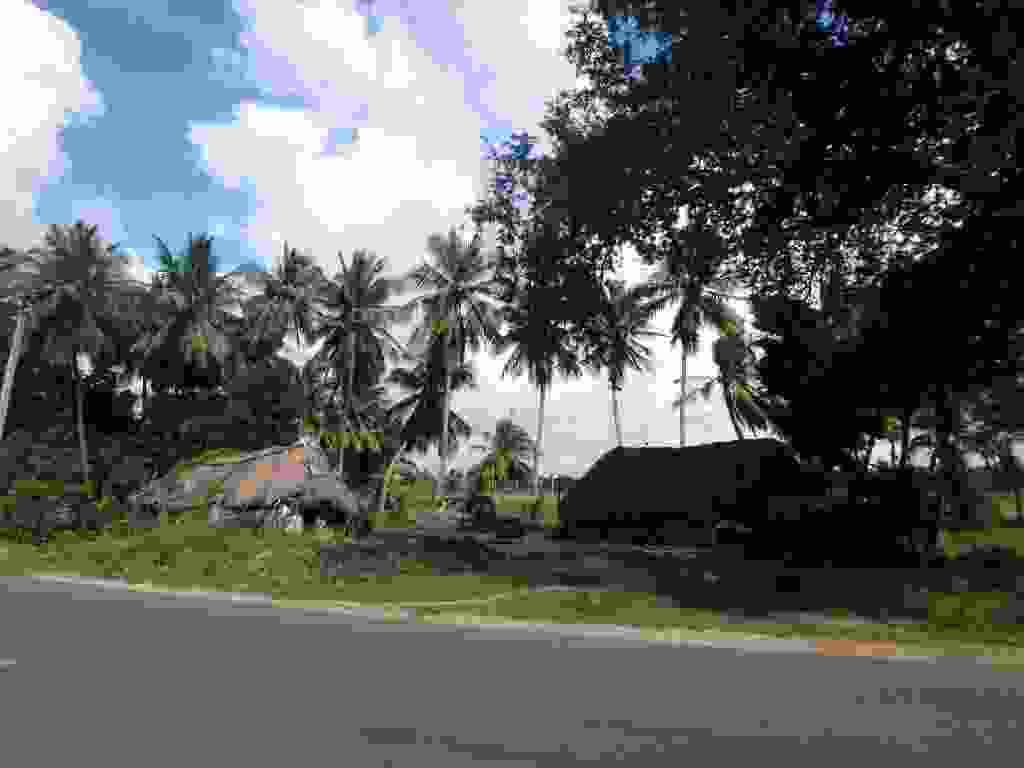
\includegraphics[width=\mywidth]{../wp-content/uploads/2015/11/wpid-oi000546-1024x768.jpg} \end{center}
\begin{center} 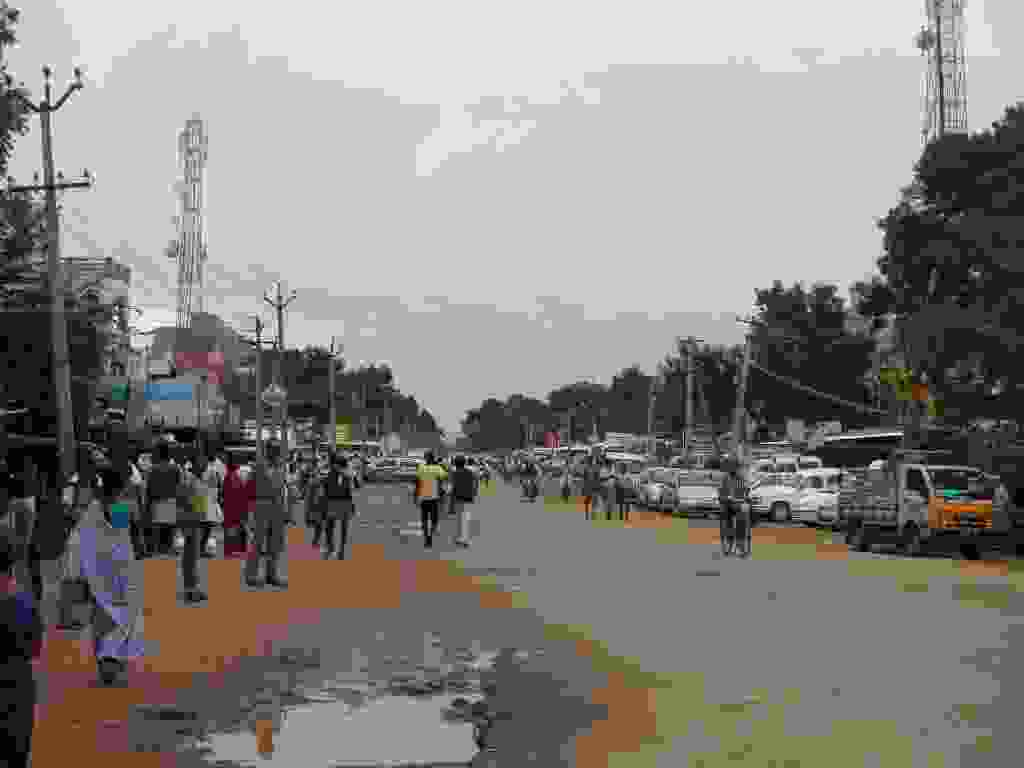
\includegraphics[width=\mywidth]{../wp-content/uploads/2015/11/wpid-oi000549-1024x768.jpg} \end{center}

 Arrivée sous une forte pluie, je vois ce que veut dire mousson. 
\begin{center} 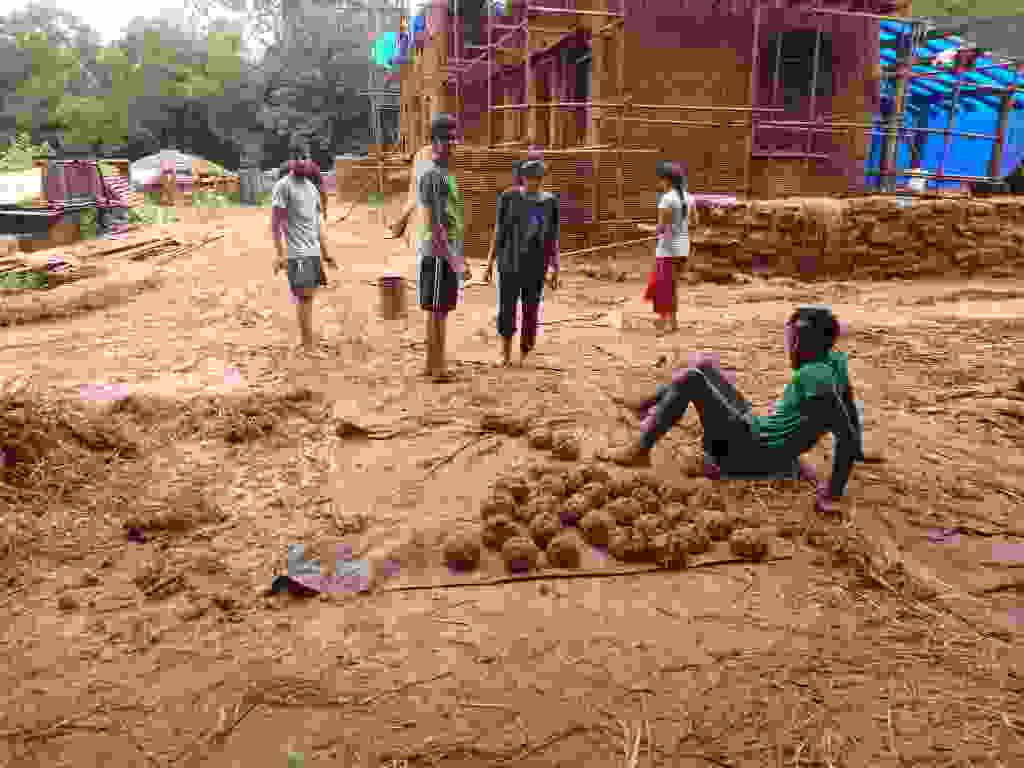
\includegraphics[width=\mywidth]{../wp-content/uploads/2015/11/wpid-oi000552-1024x768.jpg} \end{center}

\pagebreak
 Je trouve une Guest House tenue par un français. En me voyant arriver en vélo il me raconte l'histoire de son père qui a le record de la plus longue échappée en solitaire au Tour de France. 
\begin{center} 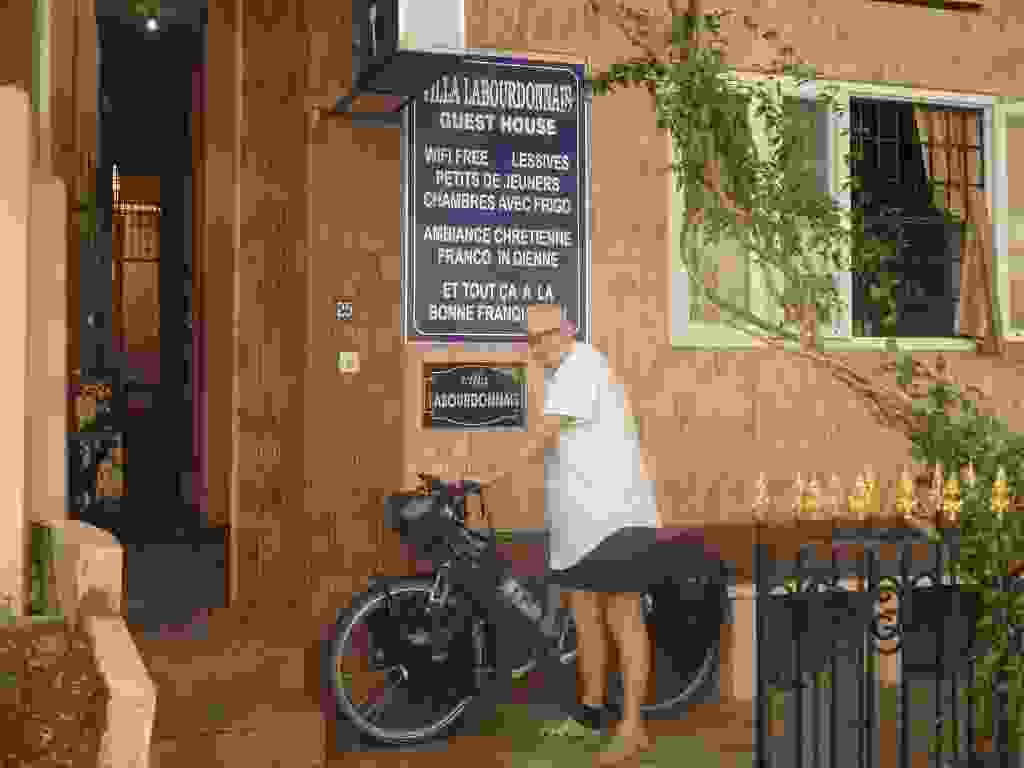
\includegraphics[width=\mywidth]{../wp-content/uploads/2015/11/wpid-oi000597-1024x768.jpg} \end{center}

 La Guest House est dans la ville blanche, partie coloniale de Pondichéry au bord de la mer. 
\begin{center} 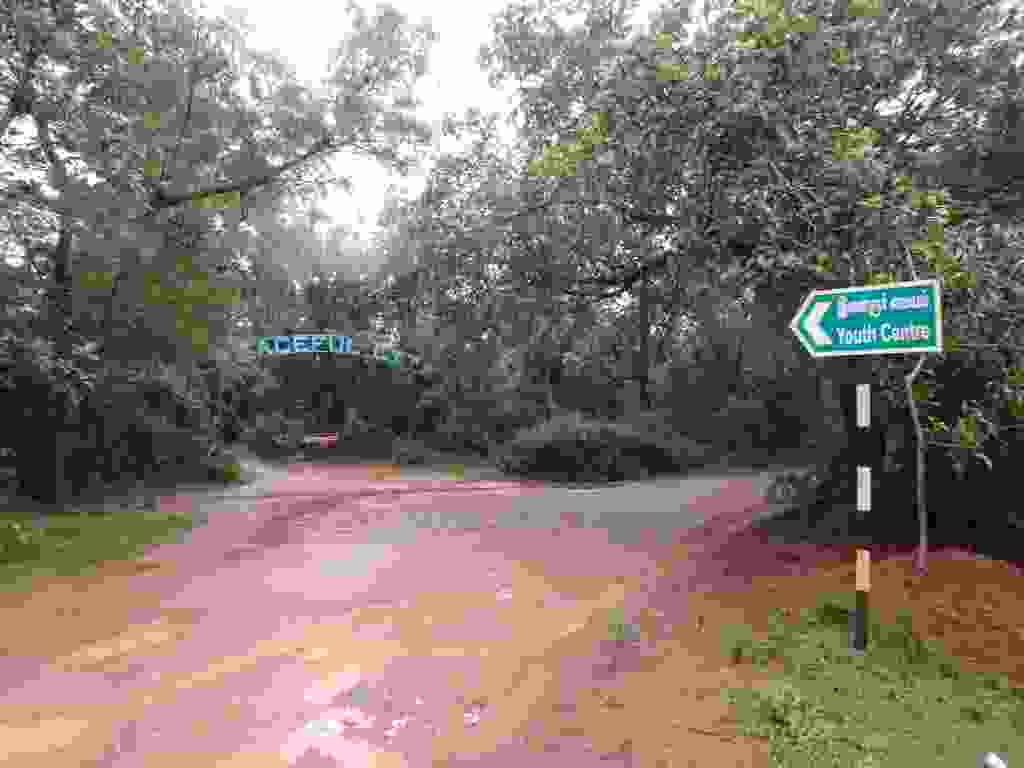
\includegraphics[width=\mywidth]{../wp-content/uploads/2015/11/wpid-oi000558-1024x768.jpg} \end{center}
\begin{center} 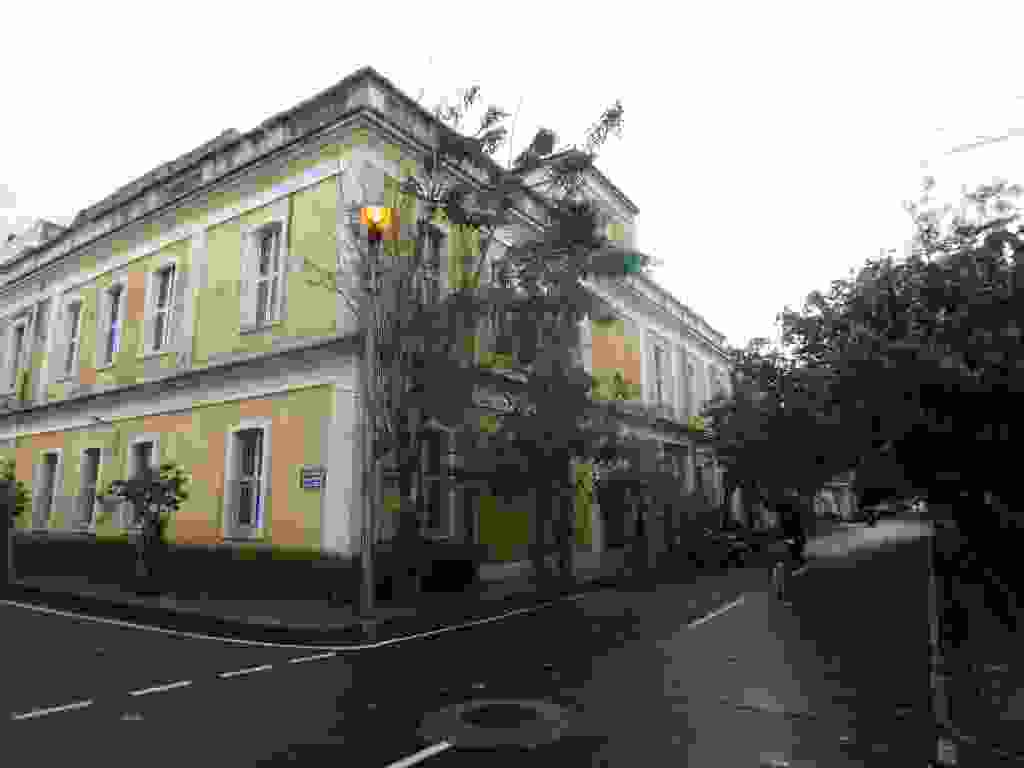
\includegraphics[width=\mywidth]{../wp-content/uploads/2015/11/wpid-oi000554-1024x768.jpg} \end{center}
\begin{center} 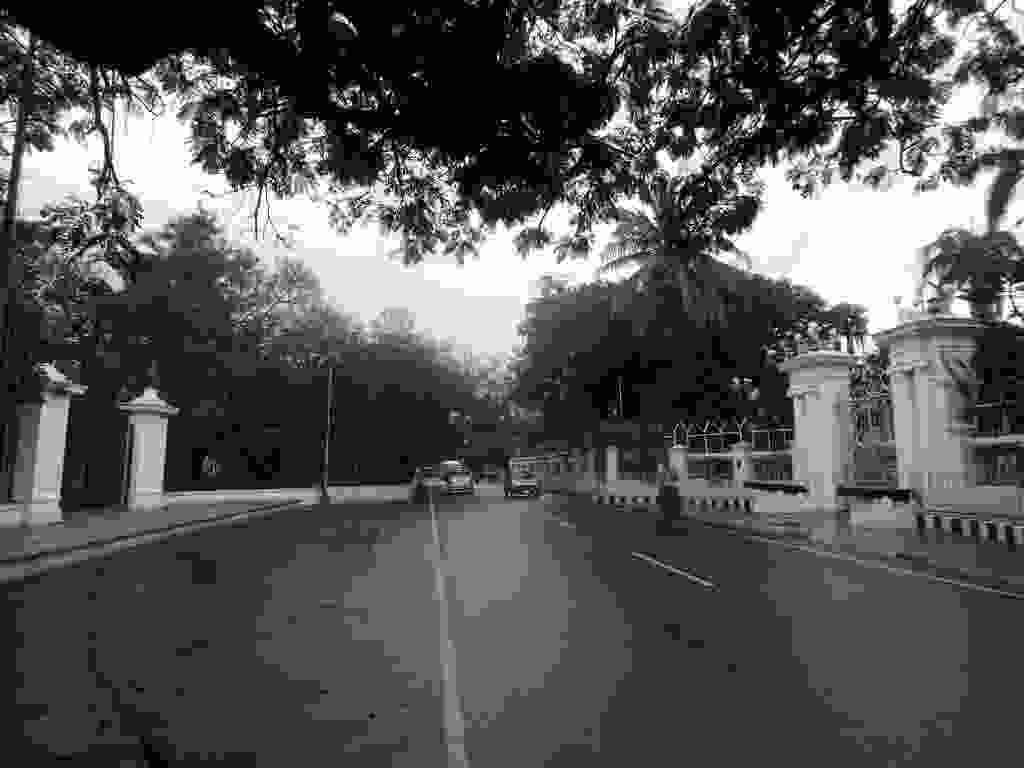
\includegraphics[width=\mywidth]{../wp-content/uploads/2015/11/wpid-oi000556-1024x768.jpg} \end{center}
\begin{center} 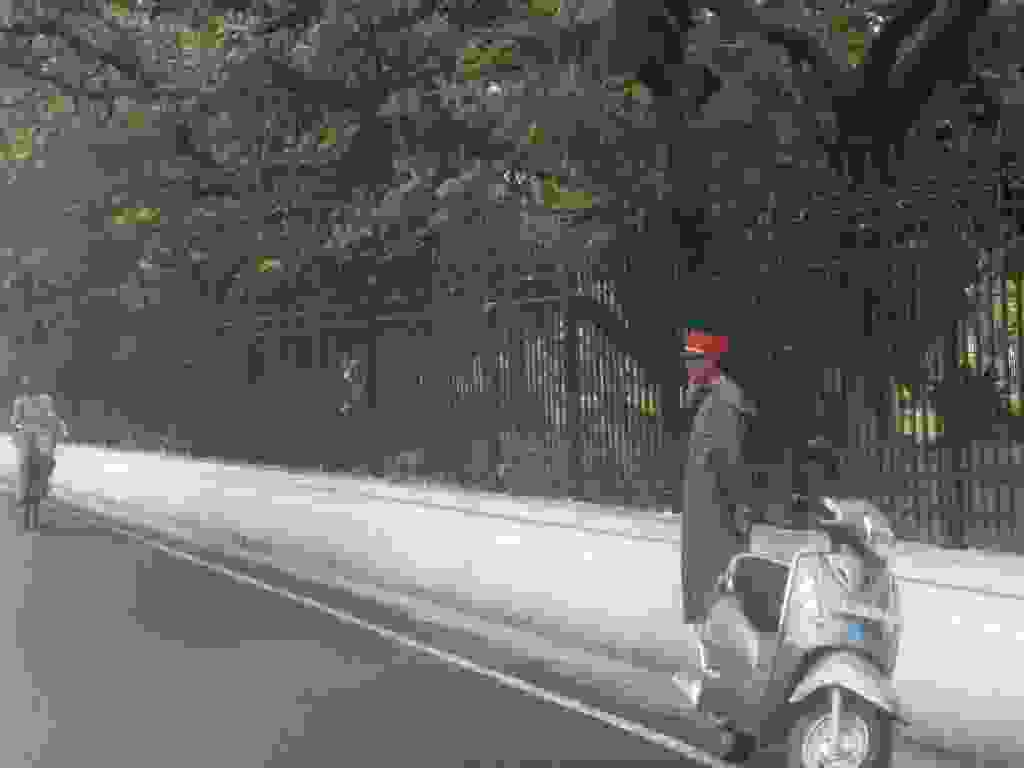
\includegraphics[width=\mywidth]{../wp-content/uploads/2015/11/wpid-oi000557-1024x768.jpg} \end{center}

 Grand bazar. 
\begin{center} 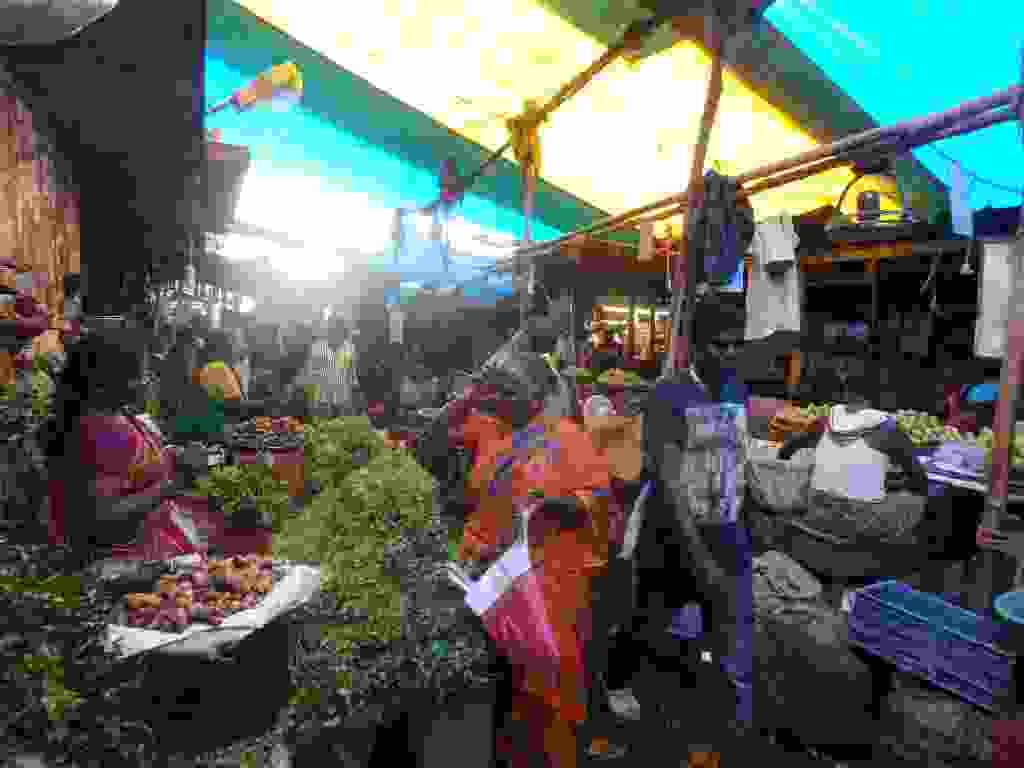
\includegraphics[width=\mywidth]{../wp-content/uploads/2015/11/wpid-oi0002675-1024x768.jpg} \end{center}

\pagebreak
 Je passe 1 jour à Mahabalipuram, 100km au nord, pour voir les temples sculptés dans d'énormes blocs de pierres. 
\begin{center} 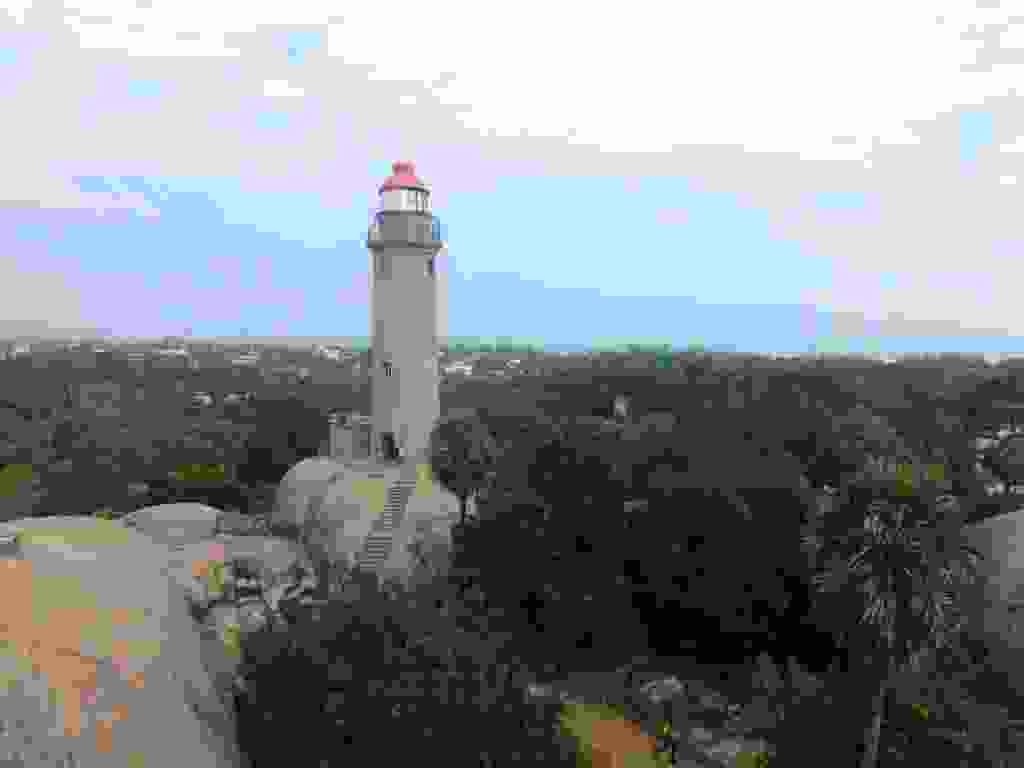
\includegraphics[width=\mywidth]{../wp-content/uploads/2015/11/wpid-oi000573-1024x768.jpg} \end{center}
\begin{center} 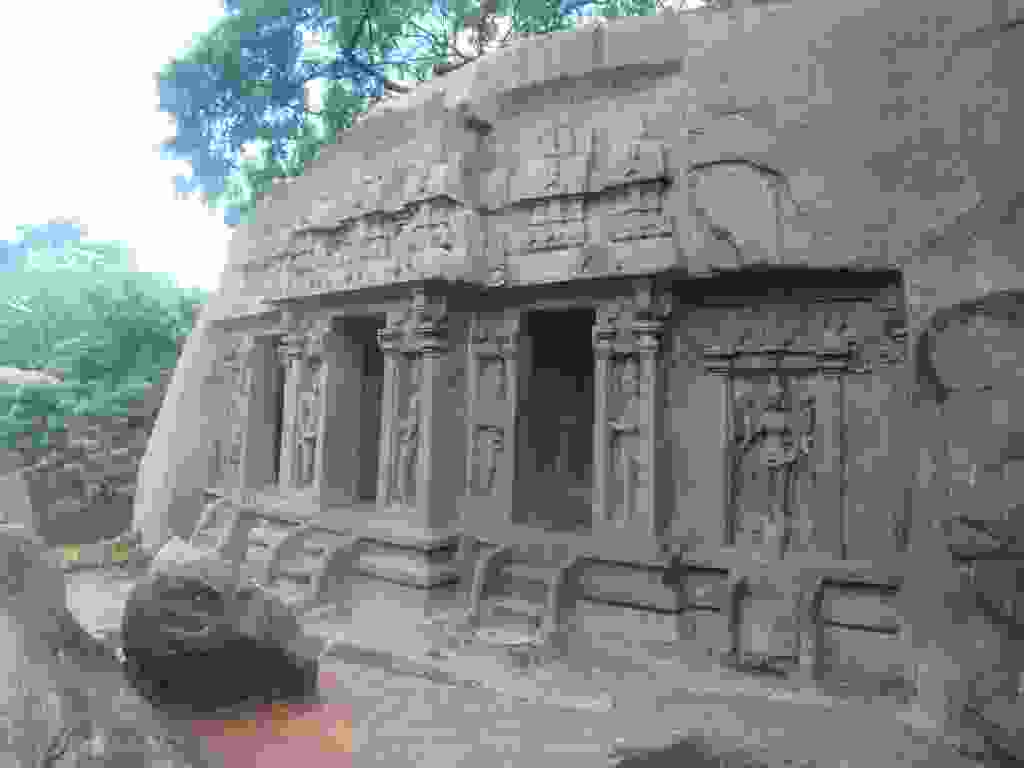
\includegraphics[width=\mywidth]{../wp-content/uploads/2015/11/wpid-oi000590-1024x768.jpg} \end{center}
\begin{center} 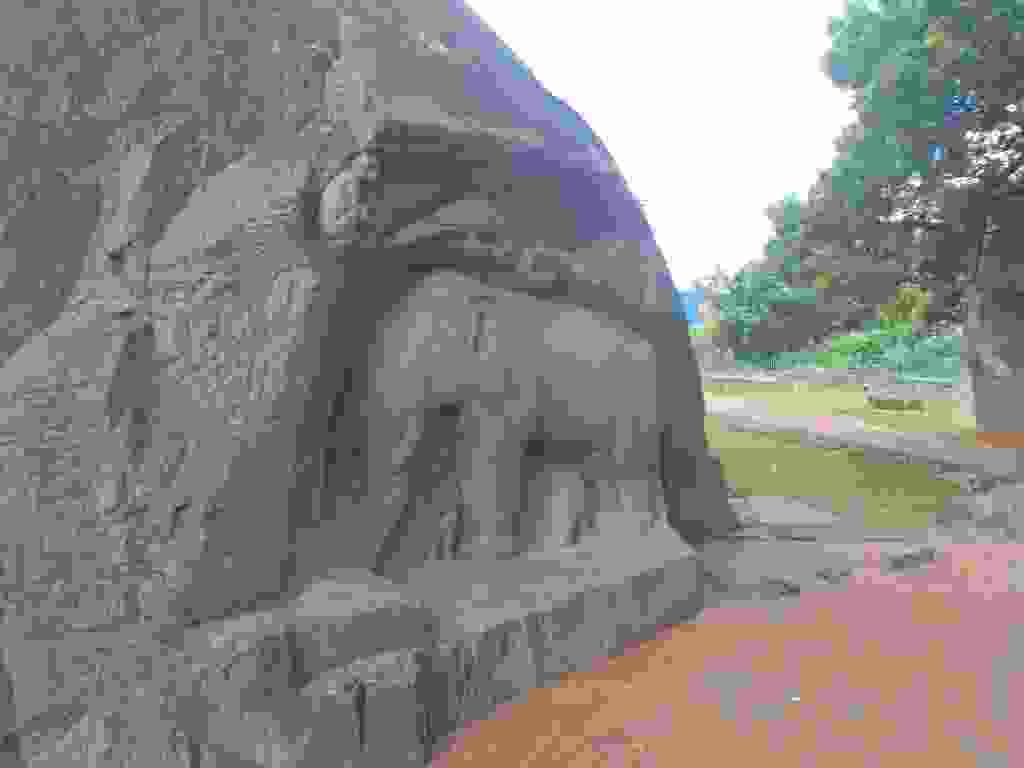
\includegraphics[width=\mywidth]{../wp-content/uploads/2015/11/wpid-oi000593-1024x768.jpg} \end{center}
\begin{center} 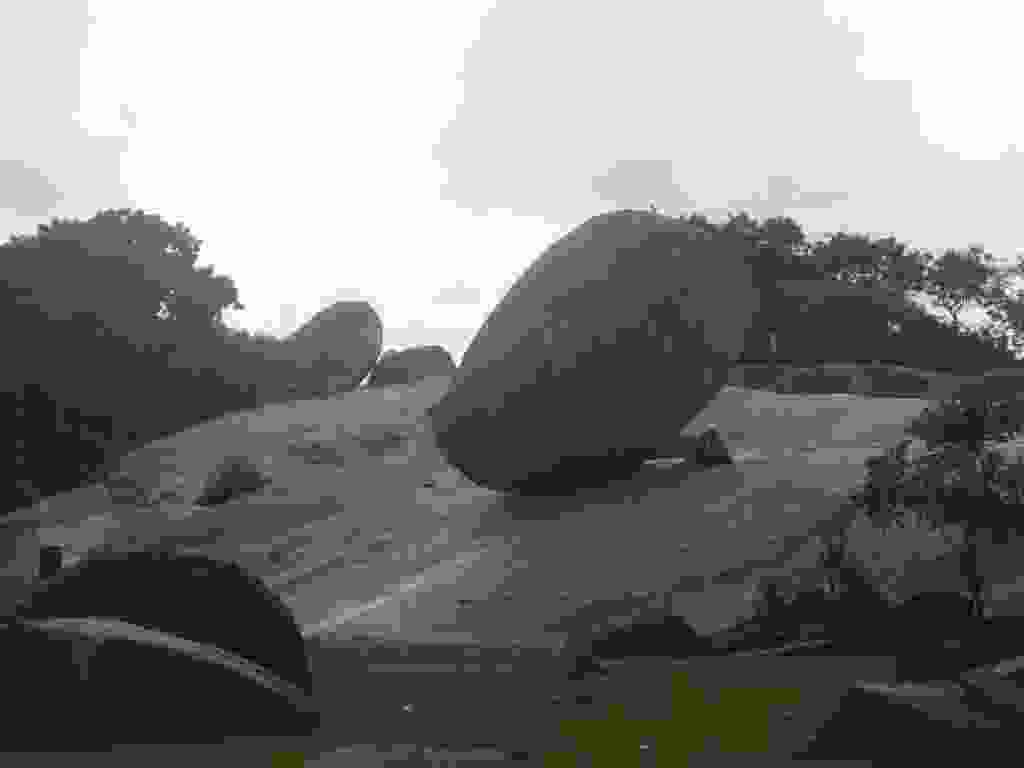
\includegraphics[width=\mywidth]{../wp-content/uploads/2015/11/wpid-oi000594-1024x768.jpg} \end{center}

\pagebreak
 Shore temple. 
\begin{center} 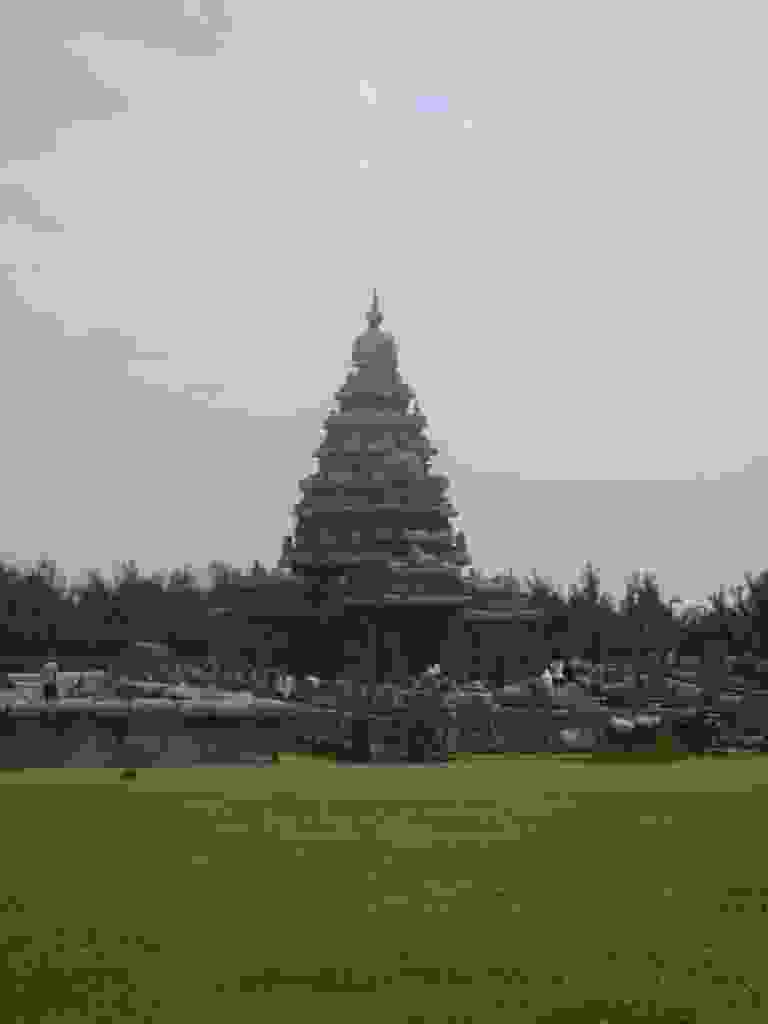
\includegraphics[height=\mywidth]{../wp-content/uploads/2015/11/wpid-oi000563-e1449029075344-768x1024.jpg} \end{center} 
\begin{center} 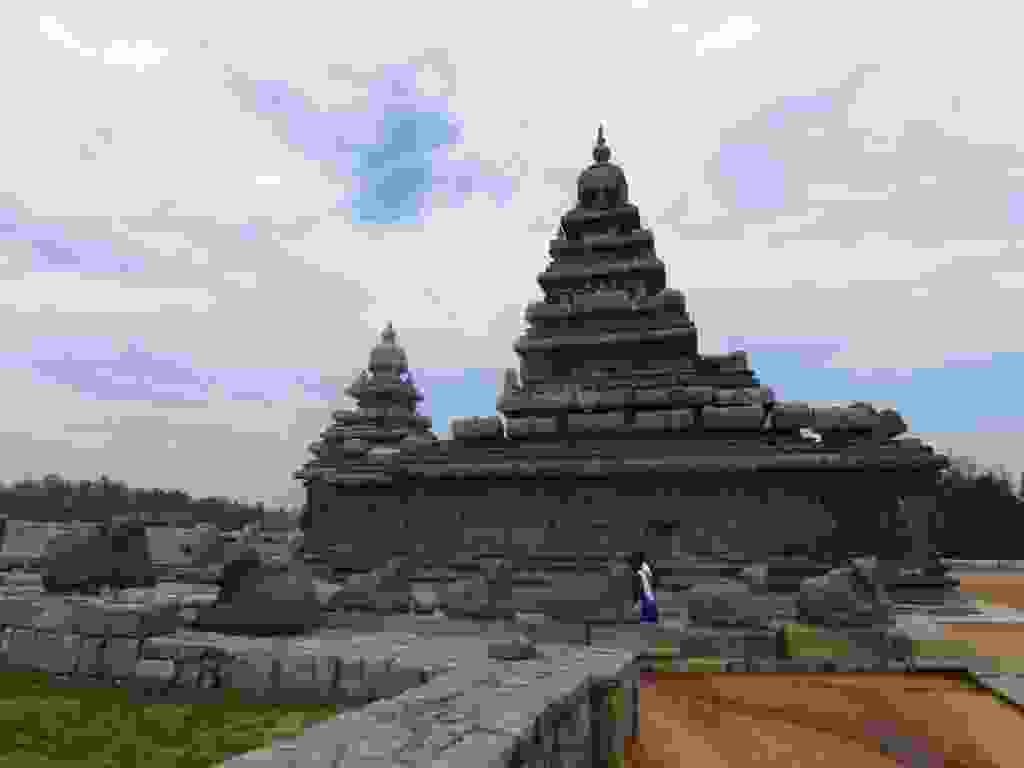
\includegraphics[width=\mywidth]{../wp-content/uploads/2015/11/wpid-oi0005292-1024x768.jpg} \end{center}
\begin{center} 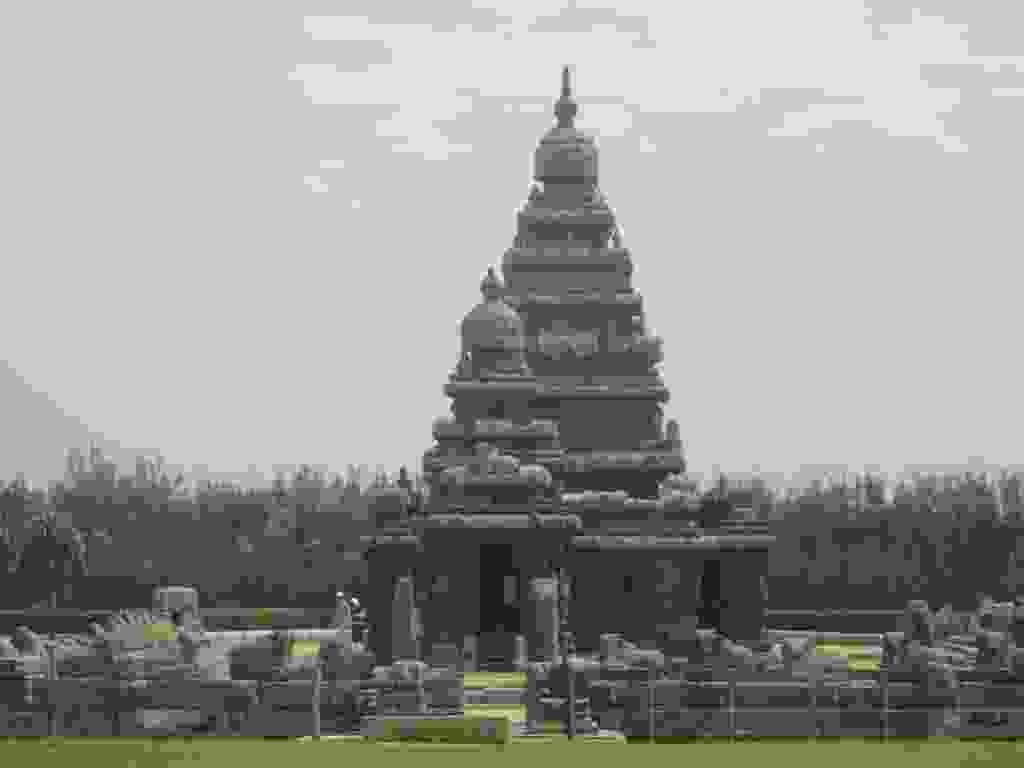
\includegraphics[width=\mywidth]{../wp-content/uploads/2015/11/wpid-oi0004723-1024x768.jpg} \end{center}

 Les 5 chariots. 
\begin{center} 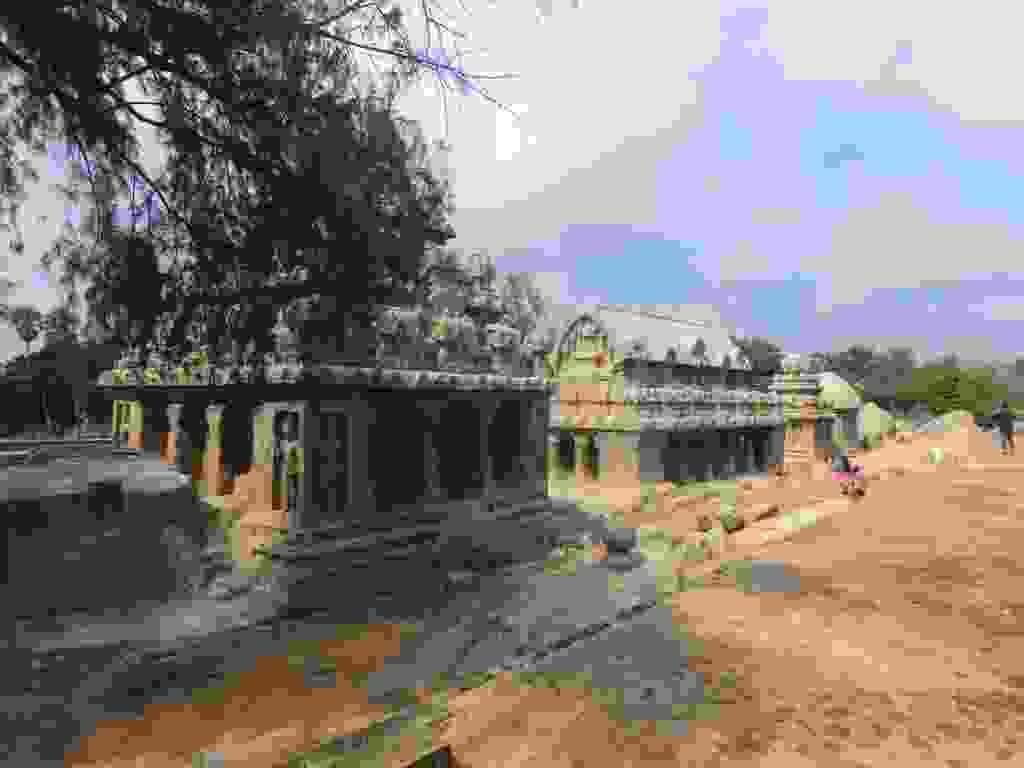
\includegraphics[width=\mywidth]{../wp-content/uploads/2015/11/wpid-oi000578-1024x768.jpg} \end{center}
\begin{center} 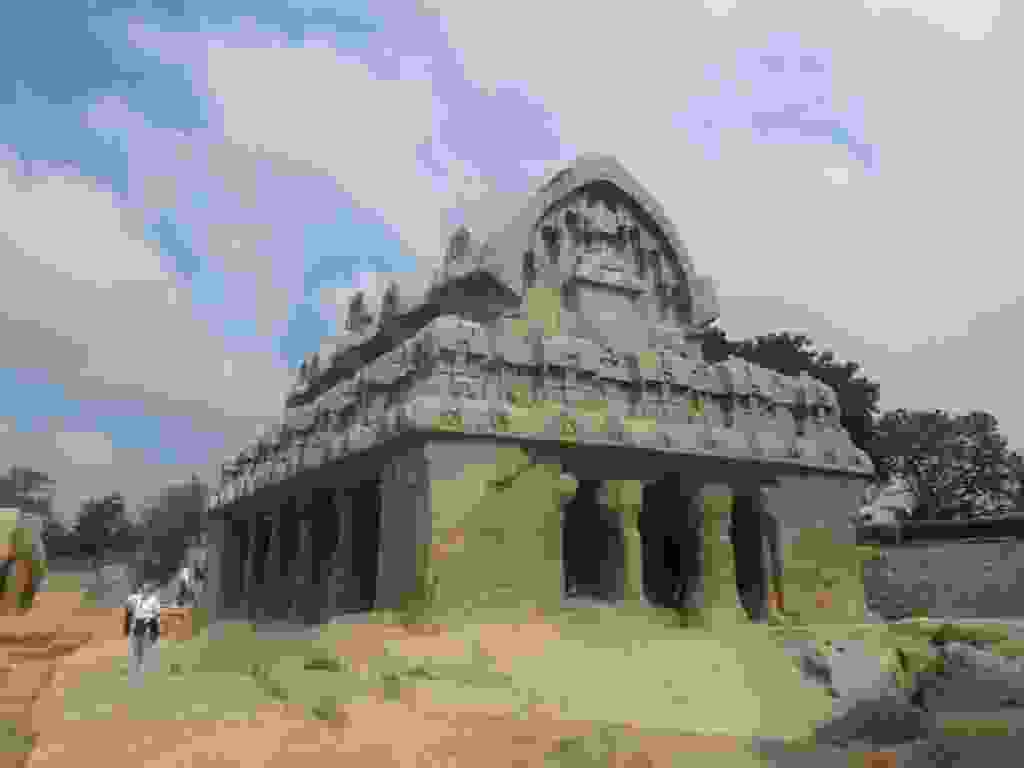
\includegraphics[width=\mywidth]{../wp-content/uploads/2015/11/wpid-oi000580-1024x768.jpg} \end{center}
\begin{center} 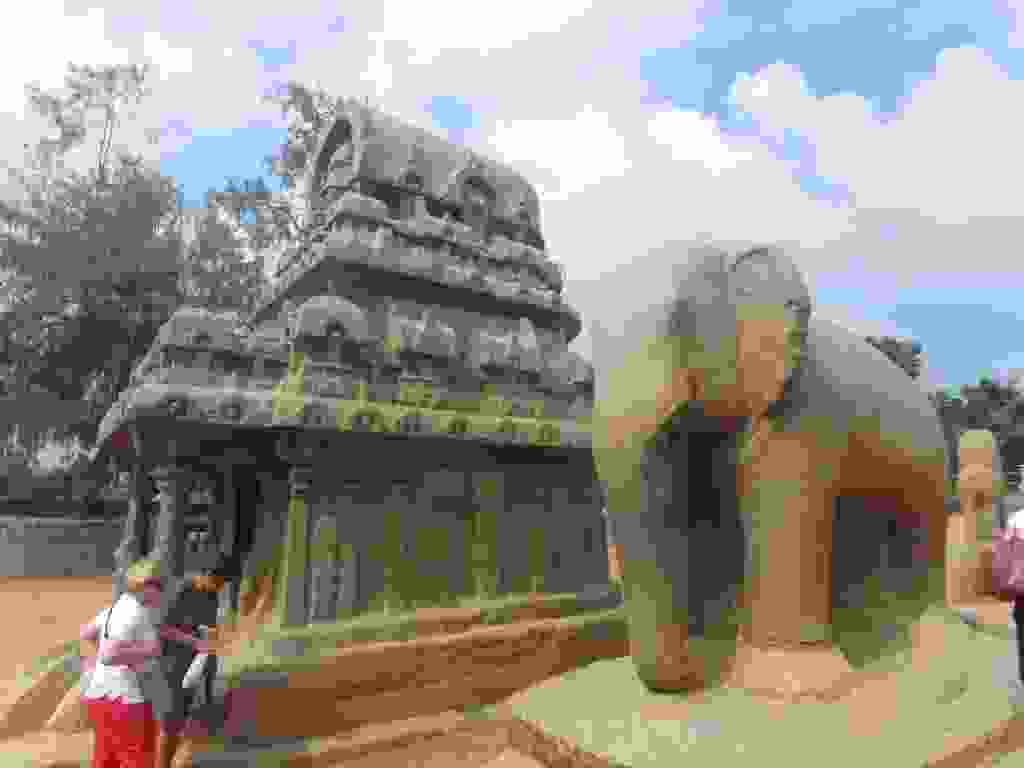
\includegraphics[width=\mywidth]{../wp-content/uploads/2015/11/wpid-oi000581-1024x768.jpg} \end{center}
\begin{center} 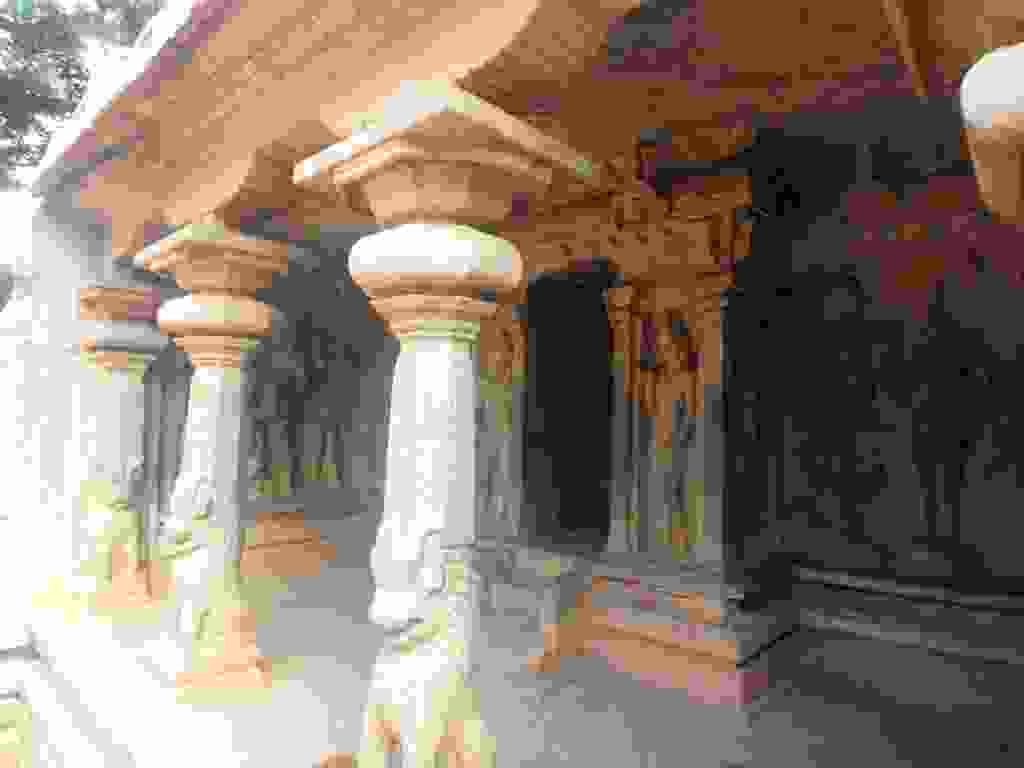
\includegraphics[width=\mywidth]{../wp-content/uploads/2015/11/wpid-oi000587-1024x768.jpg} \end{center}

 Juste avant de partir, un indien me propose de boire le thé. J'accepte et je me retrouve chez lui avec sa copine française et plusieurs amis. Un thé, un repas, quelques discussions, puis son ami qui est dans l'export de bijoux me propose une affaire : comme il y a des quotas pour l'Europe il me demande d'envoyer un colis en France en échange de 2000 €. Sans rien payer, ils s'occupent de tout. 

 J'ai déjà entendu parler d'une escroquerie avec des bijoux, du coup je refuse. 

 Et j'ai bien fait car j'ai ensuite lu sur internet plein de témoignages de gens qui ont perdu des milliers d'euros dans ce genre d'affaires.
